\documentclass[SingleSpace,12pt,Proceedings]{Serre_ASCE}

\usepackage[dvips]{graphicx}
\usepackage{amsmath}
\usepackage{amsfonts}
\usepackage{amssymb}
\usepackage[pdf]{pstricks}
\usepackage{psfrag}
\usepackage{pifont}
\usepackage{epstopdf}
%\usepackage{topcapt}
\usepackage{lscape}
\usepackage{amsthm}
\usepackage{url}
\usepackage{pifont}
\usepackage{geometry}
\usepackage{fleqn}
\usepackage{txfonts}
\usepackage{wasysym}
\usepackage{lineno}
\usepackage{enumerate}
\usepackage{url}
\usepackage{times}
\usepackage{subfigure}
\usepackage{graphicx}
\usepackage{longtable}
%\usepackage{citeref}
\usepackage[skip=0pt]{caption}

% TIME ON EVERY PAGE AS WELL AS THE FILE NAME
%\usepackage{fancyhdr}
%\usepackage{currfile}
%\usepackage[us,12hr]{datetime} % `us' makes \today behave as usual in TeX/LaTeX
%\fancypagestyle{plain}{
%\fancyhf{}
%\rfoot{\small Draft Paper \\ File Name: {\currfilename} \\ Date: {\ddmmyyyydate\today} at \currenttime}
%\lfoot{Page \thepage}
%\renewcommand{\headrulewidth}{0pt}}
%\pagestyle{plain}

\begin{document}

\title{A comparison of different order hybrid finite difference-volume methods for solving the Serre equations in conservative law form}

\author{
Jordan~Pitt,%
\thanks{Mathematical Sciences Institute, Australian National University, Canberra, ACT 0200, Australia, E-mail: Jordan.Pitt@anu.edu.au. The work undertaken by the first author was supported financially by an Australian National University Scholarship.}
\\
Christopher~Zoppou,\footnotemark[1]%
%
% Adding a second author with the same affiliation (still using \thanks):
\\
Stephen~G.~Roberts,\footnotemark[1]
}

\maketitle

\begin{abstract}
In this paper we describe first- to third-order accurate numerical methods for solving the Serre equations. These methods are described as finite difference- finite volume methods because they use a finite difference approximation and a finite volume method to solve the Serre equations in conservation law form. These models are validated and used to investigate a conjecture in the literature about the results of solving the Serre equations in the presence of steep gradients. To adequately resolve dispersive waves efficiently in problems containing steep gradients a scheme is required to be at least second-order accurate.

\end{abstract}

\KeyWords{dispersive waves, conservation laws, Serre equations, finite volume method, finite difference method}

\linenumbers

%--------------------------------------------------------------------------------
\section{Introduction} \label{intro}
Free surface flows occur in many important applications such as: tsunamis, storm surges and tidal bores. Because fluid viscosity has a negligible effect on these problems they can be modelled by the Euler equations. However, numerical methods for the Euler equations are computationally expensive when dealing with these problems over large domains. Thus various approximations to the Euler equations have been derived; one of the crudest is the shallow water wave (SWW) equations which have been used to model free surface flows in the past. However, the SWW equations assume a hydrostatic pressure distribution in a fluid column which is not fully justified in rapidly varying flows where vertical acceleration of the fluid particles becomes important. It is the vertical acceleration of these particles that produces a non-hydrostatic pressure distribution and dispersive waves which are not present in the SWW equations. Consequently, many equations have been derived as approximations to the Euler equations in shallow fluids that are less restrictive in their assumptions than the SWW equations. The Serre equations are one of these approximations to the Euler equations and are of particular interest because they do not enforce a hydrostatic pressure distribution over a fluid column allowing for fully non-linear and weakly dispersive shallow water flows \cite{Bonneton-Lannes-2009-16601}. 

The Serre equations were first derived by \citeN{Serre-F-1953-857} for flat bottom topographies in one dimension. More general equations were then derived for smooth bottom topographies in one dimension \cite{Su-Gardener-1969-536} and later smooth bottom topographies in two dimensions \cite{Green-Naghdi-1976-237}. These equations have been handled in many different ways \cite{Dutykh-2014-315,Bonneton-etal-2011-1479,Antunes-do-Carmo-etal-1993-725,Chazel-etal-2011-105,Barthelemy-2006-51-1217,Barthelemy-2007-53-1423,Clamond-2011-315}. This paper follows the decomposition of the Serre equations into conservative law form \cite{Hank-etal-2010-2034,Guyenne-etal-2014-169,Zoppou-2014} and follows the formulation of \citeN{Hank-etal-2010-2034} and \citeN{Zoppou-2014}. First-, second- and third-order accurate numerical methods are developed for solving the Serre equations in conservation law form. 

%\citeN{Zoppou-Roberts-1996} demonstrated that first- and third-order methods produce diffusive errors smearing steep gradients. While second-order methods produce dissipative errors introducing non-physical oscillations around steep gradients. Because steep gradients arise naturally in fluid flows and the Serre equations produce dispersive waves \cite{El-etal-2006} it is important that physical oscillations described by the dispersive terms are not significantly polluted by either diffusion or dissipation.

This paper aims to clear up the discrepancy between the results of \citeN{Hank-etal-2010-2034} and \citeN{El-etal-2006} by examining the behaviour of a certain dam-break problem. In particular, \citeN{Hank-etal-2010-2034} stated that their first-order method was sufficient to capture the important behaviour of the dam-break problem; this paper will test the validity of that assertion. To accomplish this first-, second- and third-order accurate methods to solve the Serre equations are constructed and validated by comparing the solutions to a known analytical solution to the Serre equations and laboratory data of flows containing steep gradients. The validated models supported the findings of \citeN{El-etal-2006}. 

%--------------------------------------------------------------------------------
\section{Serre Equations}
\label{section:Serre Equations}
The Serre equations can derived by integrating the Euler equations over the water depth, as was done by \citeN{Su-Gardener-1969-536}. They can also be derived from an asymptotic expansion of the Euler equations \cite{Bonneton-Lannes-2009-16601}. The former is more consistent with the perspective from which numerical methods will be developed in this paper while the latter is useful for identifying the appropriate regions in which to use these equations as a model of fluid flow.
\begin{figure}
\begin{center}
\includegraphics[width=7.0cm]{one-dimensional-axis_Serre.eps}
\end{center}
\caption{The notation used for one-dimensional flow governed by the Serre equation.}
\label{fig:Notation}
\end{figure}

The scenario under which the Serre approximation is made consists of a two dimensional $\textbf{x} = (x,z)$ fluid over a variable bathymetry as in Figure \ref{fig:Notation}, under the action of gravity. The water depth is $h(x,t)$ and $z_b(x)$ is the bed elevation. The fluid is subject to the pressure, $p(\textbf{x},t)$ and gravitational acceleration, $\textbf{g} = (0,g)^T$ and has a velocity $\textbf{v} = (u(\textbf{x},t),w(\textbf{x},t))$, where $u(\textbf{x},t)$ is the velocity in the $x$-coordinate and $w(\textbf{x},t)$ is the velocity in the $z$-coordinate and $t$ is time. Assuming that $z_b(x)$ is constant the Serre equations read \cite{Guyenne-etal-2014-169,Zoppou-2014}
\begin{linenomath*}
\begin{subequations}\label{eq:Serre_conservative_form}
\begin{gather}
\dfrac{\partial h}{\partial t} + \dfrac{\partial (\bar{u}h)}{\partial x} = 0,
\label{eq:Serre_continuity}
\end{gather}
\begin{gather}
\underbrace{\underbrace{\dfrac{\partial (\bar{u}h)}{\partial t} + \dfrac{\partial}{\partial x} \left ( \bar{u}^2h + \dfrac{gh^2}{2}\right )}_{\text{Shallow Water Wave Equations}} + \underbrace{\dfrac{\partial}{\partial x} \left (  \dfrac{h^3}{3} \left [ \dfrac{\partial \bar{u} }{\partial x} \dfrac{\partial \bar{u}}{\partial x} - \bar{u} \dfrac{\partial^2 \bar{u}}{\partial x^2}  - \dfrac{\partial^2 \bar{u}}{\partial x \partial t}\right ] \right )}_{\text{Dispersion Terms}} = 0}_{\text{Serre Equations}}
\label{eq:Serre_momentum}
\end{gather}
\end{subequations}
\end{linenomath*}
where $\bar{u}$ is the depth averaged velocity.
%--------------------------------------------------------------------------------
\subsection{Alternative Conservation Law Form of the Serre Equations}
\label{section:Alternative Conservation Law Form of the Serre Equations}
%--------------------------------------------------------------------------------
In \citeN{Hank-etal-2010-2034} and \citeN{Zoppou-2014} it is demonstrated that the Serre equations can be rearranged into a conservation law form, by introducing a new conserved quantity
\begin{linenomath*}
\begin{gather}
\label{eq:Gdefinition}
G = uh - h^2 \dfrac{\partial h}{\partial x} \dfrac{\partial u}{\partial x} - \frac{h^3}{3} \dfrac{\partial^2 u}{\partial x^2}.
\end{gather}
\end{linenomath*}
Consequently, \eqref{eq:Serre_conservative_form} can be rewritten as
\begin{linenomath*}
\begin{subequations}
\begin{gather}
\dfrac{\partial h}{\partial t} + \dfrac{\partial (uh)}{\partial x} = 0
\label{eq:Serrecon_continuity}
\end{gather}
and
\begin{gather}
\dfrac{\partial G}{\partial t} + \dfrac{\partial}{\partial x}\left(Gu + \dfrac{gh^2}{2} - \dfrac{2h^3}{3}\dfrac{\partial u}{\partial x}\dfrac{\partial u}{\partial x}\right) = 0
\label{eq:Serrecon_momentum}
\end{gather}
\label{eq:Serrecon}
\end{subequations}
\end{linenomath*}
where the bar over $u$ has been dropped to simplify the notation. A hybrid method can be developed for the Serre equations that solves the elliptic problem \eqref{eq:Gdefinition} for $u$ and then the conservation law \eqref{eq:Serrecon} for $h$ and $G$. This replicates the process of \citeN{Hank-etal-2010-2034} and \citeN{Zoppou-2014}.
%--------------------------------------------------------------------------------
\section{Numerically Solving the Serre Equations Written in Conservation Law Form}
\label{section:Solving the Serre Equations Written in Conservation Law Form}
%--------------------------------------------------------------------------------
There are numerous ways a numerical method could be built to solve the Serre equations in conservation law form \eqref{eq:Serrecon}. For flows that contain steep gradients the finite volume method seems the most appropriate. A finite volume method to solve \eqref{eq:Serrecon} updates the conserved quantities $h$ and $G$ over a single time step $\Delta t = t^{n+1}-t^{n}$. So that
\begin{linenomath*}
\begin{gather}
\left[\begin{array}{c}
 h^{n+1} \\
 G^{n+1} \end{array}\right] = \mathcal{L}(h^{n},G^{n},u^n,\Delta t)
\label{eq:L}
\end{gather}
\end{linenomath*}
where $\mathcal{L}$ is some numerical solver for \eqref{eq:Serrecon} and the superscript denotes the time at which a quantity is evaluated; e.g. $u^n = u(t^n)$. The complete solution also involves solving \eqref{eq:Gdefinition} for $u$ given $h$ and $G$ denoted by 
\begin{linenomath*}
\begin{gather}
u^{n+1} = \mathcal{A}(h^{n+1},G^{n+1}) .
\label{eq:A}
\end{gather}
\end{linenomath*}
%--------------------------------------------------------------------------------
\section{Solving the elliptic equation $\mathcal{A}$ for $u$}
%--------------------------------------------------------------------------------
Assuming that a discretisation in space has a fixed resolution so that $x_{i+1} - x_{i} = \Delta x$ for all $i$; allows for a simple finite difference approximation to \eqref{eq:Gdefinition} as a suitable method for $\mathcal{A}$ \cite{Hank-etal-2010-2034,Zoppou-2014}. Since the goal of this paper is to develop and compare a range of different order accurate methods for this problem both a second- and fourth-order centred finite difference approximation to \eqref{eq:Gdefinition} were used. By taking such approximations to the first- and second-order spatial derivatives the second- and fourth-order analogues of \eqref{eq:Gdefinition} are given by
\begin{linenomath*}
\begin{gather*} \tag{5a} \label{eq:Gsecondord}
G_i = u_ih_i - h_i^2 \left(\dfrac{h_{i+1} - h_{i-1}}{2\Delta x}\right) \left(\dfrac{u_{i+1} - u_{i-1}}{2\Delta x}\right) - \frac{h_i^3}{3} \left(\dfrac{u_{i+1} - 2 u_{i} + u_{i-1}}{\Delta x^2}\right)
\end{gather*}
\end{linenomath*}
and
\begin{linenomath*}
\begin{gather*} \tag{5b} \label{eq:Gfourthord}
\begin{split} 
G_i = u_ih_i - h_i^2 \left(\dfrac{-h_{i+2} + 8h_{i+1} - 8h_{i-1} + h_{i-2}}{12\Delta x}\right) \left(\dfrac{-u_{i+2} + 8u_{i+1} - 8u_{i-1} + u_{i-2}}{12\Delta x}\right) \\ - \frac{h_i^3}{3} \left(\dfrac{-u_{i+2} + 16u_{i+1} - 30u_{i} + 16u_{i-1} - u_{i-2}}{12\Delta x^2}\right)&
\end{split}
\end{gather*}
\end{linenomath*}
where the subscript denotes the spatial coordinate at which the quantity is evaluated; e.g. $u_i = u(x_i)$. Both of these can be rearranged into a matrix equation with the following form 
\begin{linenomath*}
\begin{gather*}
\left[\begin{array}{c}
  u_0 \\
  \vdots \\
  u_m \end{array}\right] = A^{-1}\left(h\right)
\left[\begin{array}{c}
 G_0 \\
 \vdots \\
 G_m \end{array}\right] =: \mathcal{A}(\boldsymbol{h},\boldsymbol{G})
\end{gather*}
\end{linenomath*}
where for a second-order approximation the matrix $A(h)$ is tri-diagonal while for a fourth-order method it is penta-diagonal.
%--------------------------------------------------------------------------------
\section{Solving the conservation law form of the Serre equations}
%--------------------------------------------------------------------------------
A finite volume method of sufficient order was developed to solve \eqref{eq:Serrecon}. Unlike finite difference methods which utilise nodal values of quantities, finite volume methods use the cell averages of the conserved quantities, for example the average water depth over a cell which spans $\left[x_{i - 1/2} , x_{i + 1/2}\right]$ is 
\begin{linenomath*}
\begin{gather*}
\bar{h}_i = \dfrac{1}{\Delta x} \int_{x_{i-\frac{1}{2}}}^{x_{i+\frac{1}{2}}} h(x,t) \, dx 
\end{gather*}
\end{linenomath*}
where $x_{i \pm 1/2} = x_i \pm \Delta x/2$. Finite volume methods update the cell averages using
\begin{linenomath*}
\begin{gather}\label{eq:FVMupdate}
\bar{U}^{n+1}_i = \bar{U}^{n}_i - \dfrac{\Delta t}{\Delta x} \left(F^n_{i+ \frac{1}{2}} - F^n_{i - \frac{1}{2}} \right)
\end{gather}
\end{linenomath*}
where $\bar{U}^{n}_i = \left[ \bar{h}^{n}_i \; \bar{G}^{n}_i \right] ^T$ is an approximation of the vector of the conserved quantities averaged over the cell at time $t^n$. While $F^n_{i\pm 1/2}$ is an approximation of the average flux over the time interval $[t^n, t^{n+1}]$ at the respective cell boundary $x_{i \pm 1/2 }$, which is obtained by solving a local Riemann problem at the cell boundaries.
%--------------------------------------------------------------------------------
\subsection{Local Riemann Problem} %
%--------------------------------------------------------------------------------
Since $\bar{U}^{n}_i$ is known for all $i$, what remains is to calculate the time averaged fluxes $F_{i \pm 1/2}$ in \eqref{eq:FVMupdate}. In \citeN{Kurganov-etal-2001-707} the time averaged inter-cell flux is approximated by
\begin{linenomath*}
\begin{gather}\label{eq:HLL_flux}
F_{i+\frac{1}{2}} = \dfrac{a^+_{i+\frac{1}{2}} f\left(q^-_{i+\frac{1}{2}}\right) - a^-_{i+\frac{1}{2}} f\left(q^+_{i+\frac{1}{2}}\right)}{a^+_{i+\frac{1}{2}} - a^-_{i+\frac{1}{2}}}  + \dfrac{a^+_{i+\frac{1}{2}} \, a^-_{i+\frac{1}{2}}}{a^+_{i+\frac{1}{2}} - a^-_{i+\frac{1}{2}}} \left [ q^+_{i+\frac{1}{2}} - q^-_{i+\frac{1}{2}} \right ]
\end{gather}
\end{linenomath*}
where $f$ is the instantaneous flux of the conserved quantity $q$ evaluated using the reconstructed values from the cells adjacent to the cell interface $x_{i + 1/2}$. While $a^-_{i+1/2}$ and $a^+_{i+1/2}$ are given by
\begin{linenomath*}
\begin{gather*}
a^-_{i+\frac{1}{2}} = \min \left[\lambda_1\left(q^-_{i + \frac{1}{2}}\right), \lambda_1\left(q^+_{i + \frac{1}{2}}\right), 0 \right]
%\label{eq:aatcelledgep}
\end{gather*}
\end{linenomath*}
and
\begin{linenomath*}
\begin{gather*}
a^+_{i+\frac{1}{2}} = \max \left[\lambda_2\left(q^-_{i + \frac{1}{2}}\right), \lambda_2\left(q^+_{i + \frac{1}{2}}\right), 0 \right]
%\label{eq:aatcelledgem}
\end{gather*}
\end{linenomath*}
where $\lambda_1$ and $\lambda_2$ are estimates of the smallest and largest eigenvalues respectively of the Jacobian, $\partial f / \partial u$.
%--------------------------------------------------------------------------------
\subsection{Propagation Speeds of a Local Shock} %
%--------------------------------------------------------------------------------
The phase speed $\upsilon_p$ of the Serre equations can be calculated by a linearisation to be
\begin{linenomath*}
\begin{gather*}
 \upsilon_p = u \pm \sqrt{gh}\sqrt{\frac{3}{h^2k^2 + 3}}
\end{gather*}
\end{linenomath*}
where $k$ is the wave number \cite{Zoppou-2014}. Thus the phase speeds of the SWW equations bound the phase speeds of the Serre equations so $\lambda_1$ and $\lambda_2$ can be defined as such
\begin{linenomath*}
\begin{gather*}
 \lambda_1 := u - \sqrt{gh} \le \upsilon_p \le u + \sqrt{gh} =: \lambda_2 .
\end{gather*}
\end{linenomath*}
%--------------------------------------------------------------------------------
\subsection{Reconstruction of Conserved Quantities} %
%--------------------------------------------------------------------------------
The quantities $q^-_{i + 1/2}$ and $q^+_{i + 1/2}$ in \eqref{eq:HLL_flux} are given by the two reconstructions at $x_{i + 1/2}$, one from the cell to the left $[x_{i - 1/2}, x_{i+ 1/2}]$ and one from the cell to the right $[x_{i + 1/2}, x_{i+ 3/2}]$ denoted by the superscripts $-$ and $+$ respectively. The order of the polynomials used to reconstruct the quantities inside the cells determines the spatial order of accuracy. Constant polynomials result in a first-order method \cite{Godunov-1959-271}. Similarly first- and second-degree polynomials result in second- and third-order accurate methods respectively. 

For a zero-degree polynomial the interpolant has the value $\bar{q}_i$ at $x_i$, this is also the case for linear interpolation functions. For the zero-degree case the interpolants are fully determined i.e $q^{+}_{i - 1/2} = \bar{q}_i = q^{-}_{i+ 1/2}$ and monotinicity preserving. There are a variety of ways to construct higher-degree interpolants not all of which are necessarily monotoncity preserving, which can result in the introduction of numerical oscillations during the reconstruction process. To suppress these non-physical oscillations in higher order methods limiting must be implemented. For the second-order method the minmod limiter was used as in \citeN{Kurganov-etal-2001-707}. While for the third-order method the Koren limiter was used \cite{Koren-1993}. This results in the following reconstruction scheme for the second-order method
\begin{linenomath*}
\begin{gather*}
q^-_{i + \frac{1}{2}} =  \bar{q}_i + a_i \frac{\Delta x}{2}
\end{gather*}
and
\begin{gather*}
q^+_{i + \frac{1}{2}} =  \bar{q}_{i+1} - a_{i + 1} \frac{\Delta x}{2}
\end{gather*}
where
\begin{gather*}
a_i = \text{minmod}\left\lbrace\theta \frac{\bar{q}_{i+1} - \bar{q}_{i}}{\Delta x}, \frac{\bar{q}_{i+1} - \bar{q}_{i-1}}{2\Delta x} ,\theta \frac{\bar{q}_{i} - \bar{q}_{i-1}}{\Delta x}\right\rbrace \quad \text{for} \; \theta \in \left[1,2\right].
\end{gather*}
\end{linenomath*}
While for the third-order method the reconstruction scheme is
\begin{linenomath*}
\begin{gather*}
q^-_{i + \frac{1}{2}} = \bar{q}_i + \frac{1}{2}\phi^-\left(r_i\right)\left(\bar{q}_i -\bar{q}_{i-1} \right)
\end{gather*}
and
\begin{gather*}
q^+_{i + \frac{1}{2}} = \bar{q}_{i+1} - \frac{1}{2}\phi^+\left(r_{i+1}\right)\left(\bar{q}_{i+1} -\bar{q}_{i} \right)
\end{gather*}
where
\begin{gather*}
\phi^-\left(r_i\right) = \max\left[0, \min\left[2 r_i, \frac{1 + 2r_i}{3},2\right]\right],
\end{gather*}
\begin{gather*}
\phi^+\left(r_i\right) = \max\left[0, \min\left[2 r_i, \frac{2 + r_i}{3},2\right]\right]
\end{gather*}
and
\begin{gather*}
r_i = \frac{\bar{q}_{i+1} - \bar{q}_{i} }{\bar{q}_{i} - \bar{q}_{i-1}}.
\end{gather*}
\end{linenomath*}

%--------------------------------------------------------------------------------
\subsection{Reconstruction of $u$} %
%--------------------------------------------------------------------------------
The finite difference methods for \eqref{eq:A} return $u$ as nodal values at the cell centres thus the reconstruction of $u$ at the cell edges is different to the process described above for $h$ and $G$. Assuming $u$ is smooth a simple interpolation can be used without limiting. For first- and second-order methods the linear interpolation between the two neighbouring cell centres was used which results in the cell edge value being the average of the two neighbouring cell centre values. For the third-order method the cubic that interpolates the 4 neighbouring cell centres was used. This resulted in the following for first- and second-order
\begin{linenomath*}
\begin{gather*} %\label{eq:fforheightp}
u_{i+ \frac{1}{2}} = \frac{u_{i+1} + u_{i}}{2}
\end{gather*}
\end{linenomath*}
and for third-order
\begin{linenomath*}
\begin{gather*} %\label{eq:fforheightp}
u_{i+ \frac{1}{2}} =\frac{-3u_{j+2} + 27u_{j+1} + 27u_j - 3u_{j-1}}{48}.
\end{gather*}
\end{linenomath*}



%--------------------------------------------------------------------------------
\subsection{Fully discrete approximations to the instantaneous flux $f(q^{\pm}_{i + \frac{1}{2}})$} %
%--------------------------------------------------------------------------------
For water depth, the fully discrete approximation to $f(h^\pm_{i + 1/2})$ in \eqref{eq:Serrecon_continuity} is given by
\begin{linenomath*}
\begin{gather*} %\label{eq:fforheightp}
f\left(h^\pm_{i + \frac{1}{2}}\right) = u^\pm_{i + \frac{1}{2}} h^\pm_{i + \frac{1}{2}}
\end{gather*}
\end{linenomath*}
which is independent of the order of accuracy of the method. 

The flux $f(G^\pm_{i + 1/2})$ is more complicated because of the derivative term in \eqref{eq:Serrecon_momentum}  and is given by
\begin{linenomath*}
\begin{gather*} %\label{eq:fforGp}
f\left(G^\pm_{i + \frac{1}{2}}\right)= u^\pm_{i + \frac{1}{2}} G^\pm_{i + \frac{1}{2}} + \frac{g}{2} \left(h^\pm_{i + \frac{1}{2}} \right)^2 - \frac{2}{3} \left(h^\pm_{i + \frac{1}{2}} \right)^3 \left[\left(\frac{\partial u}{\partial x}\right)_{i + \frac{1}{2}}\right]^2.
\end{gather*}
\end{linenomath*}
The first-, second- and third-order approximations to the derivative term can be obtained by taking the derivative of the interpolating polynomial used in the reconstruction of $u$. Thus the following approximations to the derivatives were obtained, for the first- and second-order method
\begin{linenomath*}
\begin{gather*} %\label{eq:derivdisco1p}
\left(\frac{\partial u}{\partial x}\right)_{i + \frac{1}{2}} = \frac{ u_{i + 1} - u_{i}}{\Delta x}
\end{gather*}
\end{linenomath*}
and for the third-order method
\begin{linenomath*}
\begin{gather*} %\label{eq:derivdisco3p}
%idx*i24*(-u[i+2] + 27*u[i+1] - 27*u[i] + u[i-1]);
\left(\frac{\partial u}{\partial x}\right)_{i + \frac{1}{2}} = \frac{ -u_{i + 2} + 27u_{i +1}  -27 u_{i} + u_{i-1}  }{24\Delta x} .
\end{gather*}
\end{linenomath*}
 %--------------------------------------------------------------------------------
\subsection{Transforming between nodal values and cell averages} %
%--------------------------------------------------------------------------------
The operator $\mathcal{L}$ given by \eqref{eq:FVMupdate} uses cell averages while the operator $\mathcal{A}$ given by \eqref{eq:Gsecondord} and \eqref{eq:Gfourthord} uses nodal values at the cell centres. Therefore, a transformation from the cell averages to the nodal values is required. For the first- and second-order methods this distinction is trivial since $\bar{q}_i = q_i$. However, for the third-order method this is a very important distinction and failure to handle this correctly will result in a loss of accuracy. 

A quadratic polynomial that gives the correct cell averages for the cell centred at $x_i$ and its two neighbours satisfies this equation
\begin{linenomath*}
\begin{gather*} %\label{eq:midtoca}
q_i = \frac{- \bar{q}_{i+1} + 26\bar{q}_{i} - \bar{q}_{i-1}}{24}.
\end{gather*}
\end{linenomath*}
This is a tri-diagonal matrix equation that transforms from cell averages to nodal values with third-order accuracy and is denoted by $\mathcal{M}$. The inverse transformation $\mathcal{M}^{-1}$ denotes the solution of the tri-diagonal matrix equation given nodal values resulting in cell averages which is also third-order accurate. For the first- and second-order schemes $\mathcal{M}$ is the identity matrix. This completes the solution of the Serre equations \eqref{eq:Gdefinition} and \eqref{eq:Serrecon} with the following process denoted by $\mathcal{H}$
\begin{linenomath*}
\begin{gather*}
\mathcal{H}\left(\boldsymbol{\bar{U}}^n,\Delta t \right) = \left\lbrace 
\begin{array}{c c c} 
	\boldsymbol{U}^n &=& \mathcal{M}\left(\boldsymbol{\bar{U}}^n\right) \\
	\boldsymbol{u}^n &=& \mathcal{A}\left(\boldsymbol{U}^n\right) \\
	\boldsymbol{\bar{U}}^{n+1} &=& \mathcal{L}\left(\boldsymbol{\bar{U}}^{n},\boldsymbol{u}^n,\Delta t\right)							
\end{array} \right. .
\end{gather*}
\end{linenomath*}
%--------------------------------------------------------------------------------
\subsection{Strong-Stability-Preserving Runge-Kutta Scheme} %
%--------------------------------------------------------------------------------
The process above is first-order accurate in time. This paper will use the strong stability Runge-Kutta steps described in \citeN{Gottlieb-etal-2009-251} to construct fully second- and third-order accurate methods using linear combinations of $\mathcal{H}$. This leads to the following processes, for the first-order method
\begin{linenomath*}
\begin{align*}
\boldsymbol{\bar{U}}^{n+1} &= \mathcal{H}\left(\boldsymbol{\bar{U}}^{n},\Delta t\right)
\end{align*}
\end{linenomath*}
the second-order method
\begin{linenomath*}
\begin{align*}
\boldsymbol{\bar{U}}^{\left(1\right)} &= \mathcal{H}\left(\boldsymbol{\bar{U}}^{n},\Delta t\right), \\
\boldsymbol{\bar{U}}^{\left(2\right)} &= \mathcal{H}\left(\boldsymbol{\bar{U}}^{\left(1\right)},\Delta t\right), \\
\boldsymbol{\bar{U}}^{n+1} &=\frac{1}{2}\left(\boldsymbol{\bar{U}}^{\left(1\right)} + \boldsymbol{\bar{U}}^{\left(2\right)}  \right)
\end{align*}
%\label{eq:SSPRK2}
\end{linenomath*}
and the third-order method
\begin{linenomath*}
\begin{align*}
\boldsymbol{\bar{U}}^{\left(1\right)} &= \mathcal{H}\left(\boldsymbol{\bar{U}}^{n},\Delta t\right), \\
\boldsymbol{\bar{U}}^{\left(2\right)} &= \mathcal{H}\left(\boldsymbol{\bar{U}}^{\left(1\right)},\Delta t\right), \\
\boldsymbol{\bar{U}}^{\left(3\right)} &= \frac{3}{4}\boldsymbol{\bar{U}}^{n} + \frac{1}{4}\boldsymbol{\bar{U}}^{\left(2\right)} , \\
\boldsymbol{\bar{U}}^{\left(4\right)} &= \mathcal{H}\left(\boldsymbol{\bar{U}}^{\left(3\right)},\Delta t\right), \\
\boldsymbol{\bar{U}}^{n+1} &= \frac{1}{3}\boldsymbol{\bar{U}}^{n} + \frac{2}{3}\boldsymbol{\bar{U}}^{\left(4\right)}.
\end{align*}
%\label{eq:SSPRK3}
\end{linenomath*}
%--------------------------------------------------------------------------------
\subsection{Stability Constraint} %
%--------------------------------------------------------------------------------
A necessary condition for stability of all these explicit methods based on the finite volume method is the Courant-Friedrichs-Lewy condition \cite{Courant-etal-1928-32} which states that for each cell
\begin{linenomath*}
\begin{gather} \label{eq:CFLcond}
\Delta t < \dfrac{\Delta x}{2 \max\left(\left|\lambda_i\right|\right)} \, \forall i .
\end{gather}
\end{linenomath*} 
%--------------------------------------------------------------------------------
\section{Numerical Simulations}
\label{section:Numerical Simulations}
%--------------------------------------------------------------------------------
We now use these methods to solve three different problems; (i) the soliton which is an analytic solution of the Serre equations; (ii) one of the experiments conducted by \citeN{Hammack-Segur-1978-337} and (iii) a dam-break problem from \citeN{El-etal-2006} and \citeN{Hank-etal-2010-2034}. The first two will be used to validate the models, with the soliton used to confirm the order of convergence of the models. The second problem is used to validate the models using experimental data which contains flows with steep gradients. Lastly the dam-break problem will be used to compare the results of these methods with those of \citeN{El-etal-2006} and \citeN{Hank-etal-2010-2034}. The aim of which is to verify the claim of the latter that a first-order method for the Serre equations is sufficiently accurate to capture the important behaviour of the dam-break problem. 
%--------------------------------------------------------------------------------
\subsection{Soliton}
\label{section:Convergence Rate}
%--------------------------------------------------------------------------------
Currently cnoidal waves are the only family of analytic solutions to the Serre equations \cite{Carter-Cienfuegos-2010-259}. Solitons are a particular instance of cnoidal waves that travel without deformation and have been used to verify the convergence rates of the proposed methods in this paper. 

For the Serre equations the solitons have the following form
\begin{linenomath}
\begin{subequations}
\begin{gather}
h\left(x,t\right) = a_0 + a_1\text{sech}^2\left( \kappa\left(x - ct\right)\right)
\end{gather}
and
\begin{gather}
u\left(x,t\right) = c\left(1 - \dfrac{a_0}{h(x,t)} \right)
\end{gather}
where
\begin{gather}
\kappa = \dfrac{\sqrt{3a_1}}{2a_0 \sqrt{ a_0 + a_1}}
\end{gather}
and
\begin{gather}
c = \sqrt{g \left(a_0 + a_1\right)}
\end{gather}
\label{eq:sol}
\end{subequations}
\end{linenomath}
where $a_0$ and $a_1$ are input parameters that determine the depth of the quiescent water and the maximum height of the soliton above that respectively. In the simulation $a_0 = 10\text{m}$, $a_1 = 1\text{m}$ for $x\in\left[-500\text{m},1000\text{m}\right]$ and $t\in\left[0\text{s},50\text{s}\right]$. With $\Delta t = 0.5 \Delta x / \sqrt{g (a_0 + a_1)}$ which satisfies \eqref{eq:CFLcond} and $\theta = 1.2$ for the second-order reconstruction. The example results for $\Delta x = 100 /2^{6}\text{m}$ can be seen in Figure \ref{fig:solitone}.

\subfiglabelskip=0pt
\begin{figure}
\centering
\subfigure[][]{\label{fig:solitoneo1h}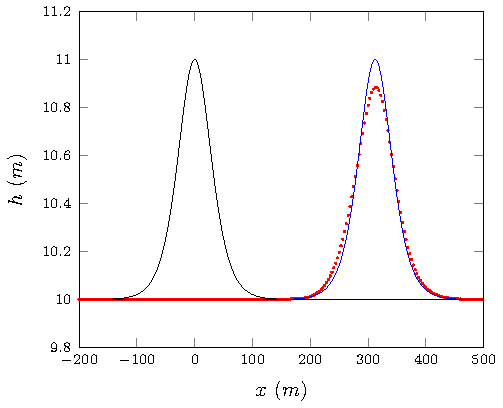
\includegraphics[width=7.0cm]{./results/soliton/ex/o1plotsolh-figure0.pdf}}
\subfigure[][]{\label{fig:solitoneo1u}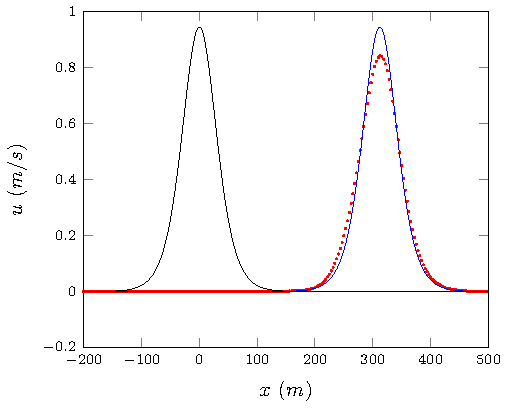
\includegraphics[width=7.0cm]{./results/soliton/ex/o1plotsolu-figure0.pdf}}
\subfigure[][]{\label{fig:solitoneo2h}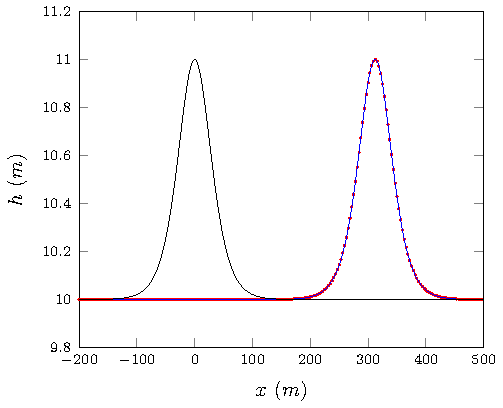
\includegraphics[width=7.0cm]{./results/soliton/ex/o2plotsolh-figure0.pdf}}
\subfigure[][]{\label{fig:solitoneo2u}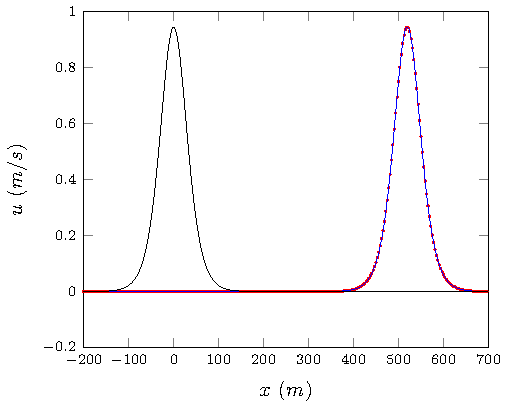
\includegraphics[width=7.0cm]{./results/soliton/ex/o2plotsolu-figure0.pdf}}
\subfigure[][]{\label{fig:solitoneo3h}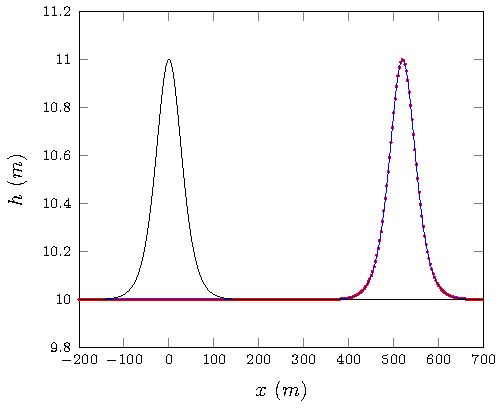
\includegraphics[width=7.0cm]{./results/soliton/ex/o3plotsolh-figure0.pdf}}
\subfigure[][]{\label{fig:solitoneo3u}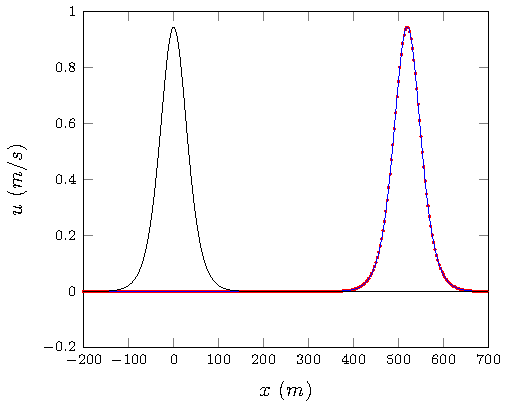
\includegraphics[width=7.0cm]{./results/soliton/ex/o3plotsolu-figure0.pdf}}
\caption{The first-, second- and third-order simulation of a soliton with $\Delta x = 100 /2^{6}\text{m}$ ($\bullet$) plotted against the analytic solution of \eqref{eq:sol} (\---) with black for $t =0\text{s}$ and blue for $t=30\text{s}$.}
\label{fig:solitone}
\end{figure}
\begin{figure}
\centering
\subfigure[][]{\label{fig:solitoncono1}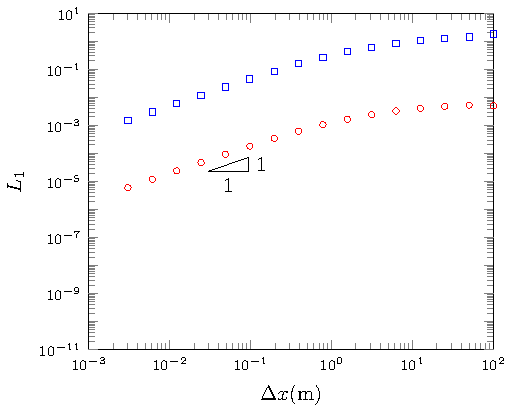
\includegraphics[width=7.0cm]{./results/soliton/con/sto1-figure0.pdf}}
\subfigure[][]{\label{fig:solitoncono2}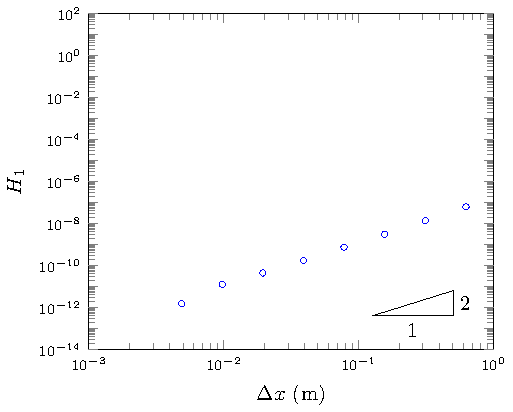
\includegraphics[width=7.0cm]{./results/soliton/con/sto2-figure0.pdf}}
\subfigure[][]{\label{fig:solitoncono3}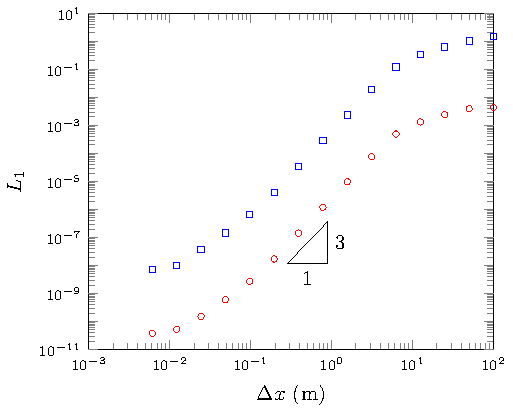
\includegraphics[width=7.0cm]{./results/soliton/con/sto3-figure0.pdf}}
\caption{Convergence of relative error using $L_1$ norm for analytic soliton solution for both $h$ ($\circ$) and $u$ ($\diamond$) for the; (a) first-, (b) second- and (c) third-order methods.}
\label{fig:solitoncon}
\end{figure} 

Figure \ref{fig:solitone} demonstrates the superiority of the second- and third-order methods compared to the first-order method. With the first-order method there is significant attenuation of the wave due to its diffusive behaviour which creates a wider wave profile and some smaller trailing waves. However, the first-order method does produce the correct speed of the wave with a small phase error. While the second- and third-order methods demonstrate no noticeable deformation resolving the soliton solution well on a relatively coarse grid with less than $500$ cells defining the actual wave.

The relative error as measured by the $L_1$-norm of the method can be seen in Figure \ref{fig:solitoncon}. For a vector $\boldsymbol{q}$ and an approximation to it $\boldsymbol{q}^*$ the relative error as measured by the $L_1$-norm is
\begin{linenomath*}
\begin{gather*}
L_1 \left(\boldsymbol{q},\boldsymbol{q}^*\right) = \frac{\sum_{i=1}^{m} |q_i - q^*_i|}{\sum_{i=1}^{m} |q_i|}.
\end{gather*}
\end{linenomath*}

Figure \ref{fig:solitoncon} demonstrates that the methods all have the correct order of convergence in both time and space. However, this order of convergence is not uniform over all $\Delta x$. When $\Delta x$ is large the actual problem is not discretised well since the cells are too large to adequately resolve the problem; this causes the observed suboptimal rate of convergence in Figure \ref{fig:solitoncon}. When $\Delta x$ is sufficiently small the numerical errors become small enough that floating point errors are significant and this can also lead to suboptimal rates of convergence as can be seen for the third-order method in Figure \ref{fig:solitoncono3}. Therefore, the order of convergence for all methods is confirmed.

Figure \ref{fig:solitoncon} also demonstrates the superiority of the second- and third-order methods over the first-order method for accuracy. The third-order method is also better than the second-order method in this respect although this difference is less pronounced. These differences have a significant impact on run-time if one wishes to run a simulation up to a desired accuracy. A comparison of the methods for such a problem is presented in Table \ref{table:runtime}.

The first-order method has a runtime two orders of magnitude greater than the second- and third-order methods. Which is reasonable because the difference in $\Delta x$ is also two orders of magnitude. This is computationally restrictive as running practical problems to a reasonable accuracy can have run times that are excessive compared to second- and third-order accurate schemes. Although the second- and third-order methods are more computationally complex than the first-order method this complexity is justified if one wants to numerically solve the Serre equations up to some desired accuracy. This also demonstrates that the second-order method is adequate compared to the third-order method for solving the Serre equations up to some desired accuracy. 

%\begin{figure}
%\centering
%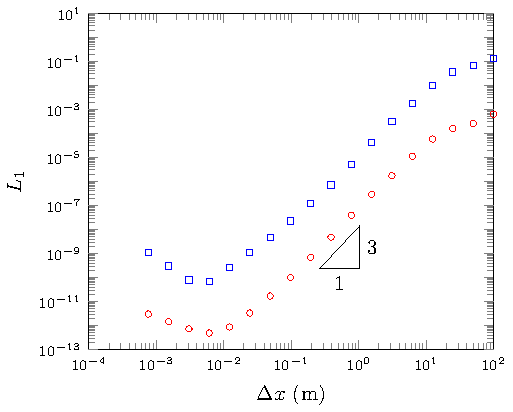
\includegraphics[width=8cm]{./results/soliton/con/sto3t1s-figure0.pdf}
%\caption{Convergence of relative error using $L_1$ norm for analytic soliton solution %for both $h$ ($\circ$) and $u$ ($\diamond$) over only a single time step}
%\label{fig:solitoncono3dt}
%\end{figure}   

%\begin{table} 
%\begin{tabular}{ | l | l | l | l | l|}
%\hline Order & $\Delta x$ (m)& $L_1$ relative error for $h$ & $L_1$ relative error for $u$ & Run Time (s) \\ 
%\hline First  & $100/2^{11}$ & $9.32715378271 \times 10^{-5}$ & $2.34320597345 \times 10^{-2}$ & $481.216886997$ \\ 
%\hline Second & $100/2^{6}$  & $5.00595847273 \times 10^{-5}$ & $1.25175521776 \times 10^{-2}$ & 2.19665694237 \\ 
%\hline Third  & $100/2^{5}$  & $7.681432554 \times 10^{-5}$ & $1.89115440455 \times 10^{-2}$ & 1.3766579628 \\
%\hline
%\end{tabular}
%\caption{Comparison of run times for different order methods to get similar relative error as measured by the $L_1$ norm for $h$}
%\label{table:runtime}
%\end{table}  

\begin{table} 
\begin{tabular}{ | l | l | l | l | l|}
\hline Order & $\Delta x$ (m)& $L_1$ relative error for $h$ & $L_1$ relative error for $u$ & Run Time (s) \\ 
\hline First  & $100/2^{10}$ & $6.85562687971 \times 10^{-5}$ & $1.28856345502 \times 10^{-2}$ & $15.2193582058$ \\ 
\hline Second & $100/2^{6}$  &  $1.28206207795\times 10^{-5}$ & $2.21972914623  \times 10^{-3}$ & $0.14813709259$ \\ 
\hline Third  & $100/2^{5}$  & $5.27876968928 \times 10^{-5}$ & $9.51078676559, \times 10^{-3}$ & 0.0947360992432 \\
\hline
\end{tabular}
\caption{Comparison of run times for different order methods to get similar relative error as measured by the $L_1$ norm for $h$}
\label{table:runtime}
\end{table} 

Figure \ref{fig:solitoncono2} and Figure \ref{fig:solitoncono3} demonstrate that the second- and third-order methods both have similar errors and Figure \ref{fig:solitone} shows that these methods resolve the problem well. Therefore, the extra effort in running a third-order method compared to a second-order method is not justified in this case. While the effort required to go from a first-order method to a second-order method is justified since attaining a similar accuracy between them requires a restrictively small $\Delta x$ for a first-order method.

%--------------------------------------------------------------------------------
\subsection{Segur Labratory Experiment}\label{Laboratory_Experiments}
%--------------------------------------------------------------------------------
\citeN{Hammack-Segur-1978-337} conducted an experiment that produced rectangular waves with the stroke of a $0.61\text{m}$ long piston flush with the wall of a wave tank $31.6\text{m}$ in length. The water height was recorded at $0\text{m}$, $5\text{m}$, $10\text{m}$, $15\text{m}$ and $20\text{m}$ from the edge of the piston furthest from the wall over time. The quiescent water height $h_1$ was $0.1\text{m}$ while the stroke of the piston caused a depression of water which was $h_0 = 0.095\text{m}$ deep. To run this as a numerical simulation the reflected problem was used. Thus the initial conditions were reflected around the origin and $h_1 - h_0$ was doubled by setting $h_0 = 0.09\text{m}$. The domain was chosen to be from $-60\text{m}$ to $60\text{m}$ and the simulation was for $t \in [0\text{s},50\text{s}]$ with $\Delta x = 0.01 \text{m}$, $\Delta t = 0.5 \Delta x / \sqrt{g h_1}$ which satisfies \eqref{eq:CFLcond} and $\theta = 1.2$ in the second-order scheme. The results of this simulation are displayed in Figures \ref{fig:Seguro1} - \ref{fig:Seguro3}.

\subfiglabelskip=0pt
\begin{figure}
\centering
\subfigure[][]{\label{fig:Seguro1p0}\includegraphics[width=7cm]{./results/segurdata/o1/plotp0-figure0.pdf}}
\subfigure[][]{\label{fig:Seguro1p5}\includegraphics[width=7cm]{./results/segurdata/o1/plotp5-figure0.pdf}}
\subfigure[][]{\label{fig:Seguro1p10}\includegraphics[width=7cm]{./results/segurdata/o1/plotp10-figure0.pdf}}
\subfigure[][]{\label{fig:Seguro1p15}\includegraphics[width=7cm]{./results/segurdata/o1/plotp15-figure0.pdf}}
\subfigure[][]{\label{fig:Seguro1p20}\includegraphics[width=7cm]{./results/segurdata/o1/plotp20-figure0.pdf}}
\caption{Comparison of the experimental results ($-$) against the first-order methods solution ($\bullet$) at $x/h_0$ : (a) $0$, (b) $50$, (c) $100$, (d) $150$ and (e) $200$.}
\label{fig:Seguro1}
\end{figure}
%
\begin{figure}
\centering
\subfigure[][]{\label{fig:Seguro2p0}\includegraphics[width=7cm]{./results/segurdata/o2/plotp0-figure0.pdf}}
\subfigure[][]{\label{fig:Seguro2p5}\includegraphics[width=7cm]{./results/segurdata/o2/plotp5-figure0.pdf}}
\subfigure[][]{\label{fig:Seguro2p10}\includegraphics[width=7cm]{./results/segurdata/o2/plotp10-figure0.pdf}}
\subfigure[][]{\label{fig:Seguro2p15}\includegraphics[width=7cm]{./results/segurdata/o2/plotp15-figure0.pdf}}
\subfigure[][]{\label{fig:Seguro2p20}\includegraphics[width=7cm]{./results/segurdata/o2/plotp20-figure0.pdf}}
\caption{Comparison of the experimental results ($-$) against the second-order methods solution ($\bullet$) at $x/h_0$ : (a) $0$, (b) $50$, (c) $100$, (d) $150$ and (e) $200$.}
\label{fig:Seguro2}
\end{figure}
%
\begin{figure}
\centering
\subfigure[][]{\label{fig:Seguro3p0}\includegraphics[width=7cm]{./results/segurdata/o3/plotp0-figure0.pdf}}
\subfigure[][]{\label{fig:Seguro3p5}\includegraphics[width=7cm]{./results/segurdata/o3/plotp5-figure0.pdf}}
\subfigure[][]{\label{fig:Seguro3p10}\includegraphics[width=7cm]{./results/segurdata/o3/plotp10-figure0.pdf}}
\subfigure[][]{\label{fig:Seguro3p15}\includegraphics[width=7cm]{./results/segurdata/o3/plotp15-figure0.pdf}}
\subfigure[][]{\label{fig:Seguro3p20}\includegraphics[width=7cm]{./results/segurdata/o3/plotp20-figure0.pdf}}
\caption{Comparison of the experimental results ($-$) against the third-order methods solution ($\bullet$) at $x/h_0$ : (a) $0$, (b) $50$, (c) $100$, (d) $150$ and (e) $200$.}
\label{fig:Seguro3}
\end{figure}

In this experiment for the positive side of the axis the initial depression causes a right going rarefaction fan and a left going shock. The shocks from both sides then reflect at the origin and so the shock and the rarefaction fan will travel in the same direction. The leading wave in all the related figures is the rarefaction fan while the trailing dispersive waves are the result of the reflected shock.  

From all the related figures it can be seen that all models show good agreement between the arrival of the first wave and the period of all the waves. While Figure \ref{fig:Seguro1} shows the first-order method is too diffusive and thus under estimates the heights of the dispersive waves. Whereas the second- and third-order methods over estimate them. This overestimation can be explained by the Serre equations ignoring viscous effects that may diffuse the dispersive waves and so the results could be considered as an upper bound on the wave heights for non-inviscid fluids. Although even without these effects these numerical methods show good agreement with the experimental data thus validating them to provide a reasonable representation of rapidly-varying flows. Additionally, it demonstrates that the oscillations observed by the produced numerical solutions of the Serre equations around steep gradients are physical and not numerical. In these simulations the numerical oscillations that the second-order method should produce \cite{Zoppou-Roberts-1996} do not have a significant influence on the physical oscillations.
%--------------------------------------------------------------------------------
\subsection{Dam-Break}
%--------------------------------------------------------------------------------
The dam-break problem used by \citeN{El-etal-2006} to compare their analysis with a second-order accurate solution of the Serre equations can be defined by
\begin{linenomath*}
\begin{gather*}
\begin{split}
h(x,0) &= \left\lbrace \begin{array}{c c}
1.8m & x < 500m\\
1.0m & x \ge 500m\\
\end{array} \right. ,\\
u(x,0) &= 0.0m/s.
\end{split}
\end{gather*}
\end{linenomath*}
With $x \in \left[0\text{m},1000\text{m}\right]$ for $t \in \left[0\text{s},30\text{s}\right]$. Where $\Delta t = 0.5 \Delta x / \sqrt{g h_1}$ which satisfies \eqref{eq:CFLcond} and $\theta = 1.2$ for the second-order scheme. This corresponds to sub-critical flow and was a situation demonstrated in \citeN{El-etal-2006} and \citeN{Hank-etal-2010-2034}. An example was plotted for $\Delta x = 100 /2^{11}\text{m}$ for all the methods and for $\Delta x = 100 /2^{17}\text{m}$ for the first-order method in Figure \ref{fig:DB}. To determine if the oscillations that occur in the solution indeed converge to some limit as $\Delta x \rightarrow 0$ multiple $\Delta x$ values were run and then the amount of variation in the solution measured. This measured how oscillatory the solution was and was used to determine the growth of the oscillations. A common way to measure this is the total variation (TV) which for $\boldsymbol{q}$ is given by
\begin{linenomath*}
\begin{gather*}
TV(\boldsymbol{q}) = \sum_{\forall i >1} |q_{i} - q_{i-1}|.
\end{gather*}
\end{linenomath*}
If the solution does indeed converge then the TV must at some point plateau, bounding the oscillations. This was indeed the findings of the experiments as can be seen by Figure \ref{fig:DBL1}. The TV increases as $\Delta x$ decreased because the models resolved more dispersive waves. As $\Delta x$ decreased further the TV plateaued and so the size and number of oscillations was bounded. Therefore, the method has not become unstable which supports the argument that the numerical methods do not introduce non-physical oscillations in the solution. Under this measure the second-order method converges rapidly to the solution of the third-order method.

\begin{figure}
\begin{center}
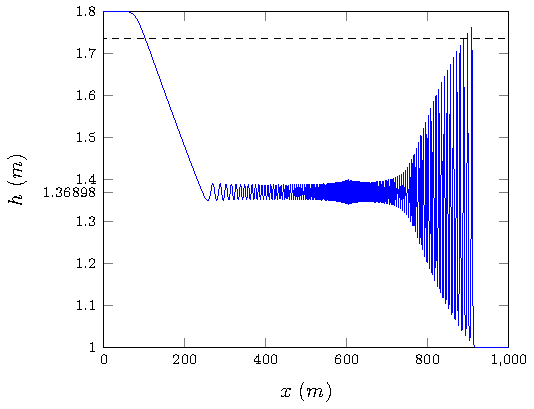
\includegraphics[width=8.0cm]{./results/dambreak/L1con/h-figure0.pdf}
\end{center}
\caption{The change in total variation (TV) of $h$ over $\Delta x$ for: ($\circ$) first- , ($\square$) second-, and ($*$) third-order methods.}
\label{fig:DBL1}
\end{figure}
\begin{figure}
\centering
\subfigure[][]{\label{fig:DBo1}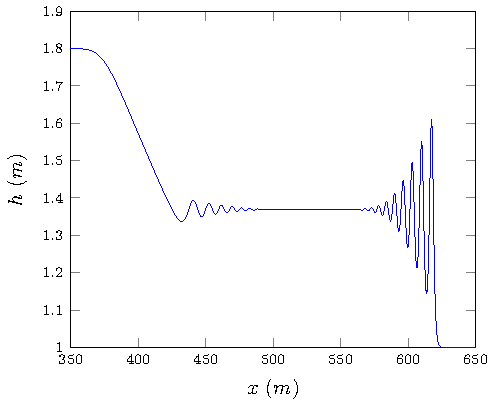
\includegraphics[width=7cm]{./results/dambreak/ex/o1-figure0.pdf}}
\subfigure[][]{\label{fig:DBo2}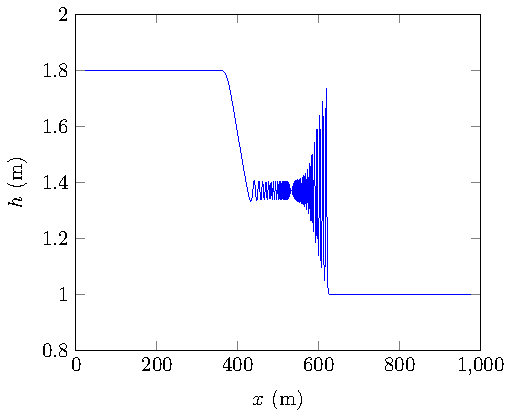
\includegraphics[width=7cm]{./results/dambreak/ex/o2-figure0.pdf}}
\subfigure[][]{\label{fig:DBo3}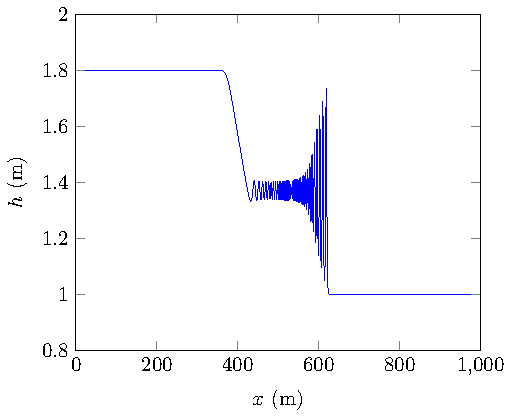
\includegraphics[width=7cm]{./results/dambreak/ex/o3-figure0.pdf}}
\subfigure[][]{\label{fig:DB1o1}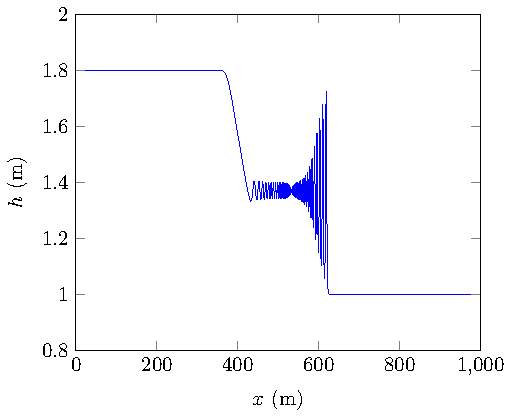
\includegraphics[width=7cm]{./results/dambreak/ex/o1-figure1.pdf}}
\caption{Solution of the dam-break problem using the (a) first-, (b) second- and (c) third-order method with $\Delta x = 100 /2^{11} \text{m}$. As well as a (d) first-order method with $\Delta x = 100 /2^{17} \text{m}$. }
\label{fig:DB}
\end{figure}

These solutions compare very well to the findings in \citeN{El-etal-2006} with both the second- and third-order methods resolving the oscillations around the ``contact discontinuity''\cite{El-etal-2006} between the rarefaction fan and the shock. In \citeN{Hank-etal-2010-2034} it was reported that for their first-order method such oscillatory behaviour was not seen. However, for the first-order method proposed in this paper when $\Delta x = 100 /2^{15}$ it was resolved as in Figure \ref{fig:DB1o1}. This validates the findings in \citeN{El-etal-2006}. Interestingly this is a much higher resolution than one needs to represent the waves themselves. It appears that the behaviour of the dispersive waves around a steep gradient is sensitive to diffusion so that even though the first-order method in Figure \ref{fig:DBo1} heuristically had enough cells to resolve most of the wave train, due to strong diffusion hardly any of the wave train was resolved. 

There is a good agreement between the second- and third-order simulations of the dam-break problem as can be seen in Figures \ref{fig:DBo2} and \ref{fig:DBo3}. Although more oscillations are resolved by the third-order method over the second-order method, there is no significant change in the resolved behaviour of this problem between the two methods. As noted in the introduction second-order accurate numerical schemes are dissipative; since the diffusive third-order method resolved the same oscillations it was demonstrated that none of the dissipative errors significantly polluted the wave train and for this problem the second-order accurate scheme is capable of resolving the problem.
%--------------------------------------------------------------------------------
\section{Conclusions}
\label{section:Conclusions}
%--------------------------------------------------------------------------------
First-, second- and third-order hybrid finite difference-volume methods were developed to solve the Serre equations written in conservative law form. The methods were then tested and validated. Firstly the order of the methods were all verified, secondly the methods steep gradient handling capability was validated by comparison with experimental data. Thirdly the behaviour of the solutions matched previous findings in \citeN{El-etal-2006}. Thus it can be concluded that these methods are all valid and they properly handle steep gradients. It was also demonstrated that for these equations although second-order is not as accurate as third-order it still provides a satisfactory method for reasonable $\Delta x$ unlike the first-order method which due to the introduction of large numerical diffusion requires computationally restrictive $\Delta x$ to produce satisfactory accuracy. Therefore; practical problems which contain steep gradients require at least a second-order method to solve the Serre equations. 
\newpage
%--------------------------------------------------------------------------------
\section{Acknowledgements}
%--------------------------------------------------------------------------------
Dr David George, Cascades Volcano Observatory, U.S. Geological Survey for providing the rectangular wave data.


%--------------------------------------------------------------------------------
\bibliography{Serre_ASCE}
%--------------------------------------------------------------------------------

\end{document}
